% Please reformat using siam11.tex.

\documentclass[twoside,leqno,twocolumn]{article}
\usepackage{ltexpprt}

%Example for automatically rescaling equations. 
% This is very tricky.
%\begin{equation}
%\label{eq:pimax}
%\resizebox{.55\textwidth}{!}{$
%\begin{split}
%P(\jtable_{2}|\set{E},\ttable) \propto &
%P(\keys = [jack,101],\it{Gr} = A, \it{Sat} = 1|\it{Int} = \class, \it{Rank} = 1, \it{Rat} = 3, \it{Diff}=1)\\
%\times & P(\keys = [jack,102],\it{Gr} = B, \it{Sat} = 2|\it{Int} = \class, \it{Rank} = 1, \it{Rat} = 2, \it{Diff}=2).
%\end{split}$
%}
%\end{equation}

%\usepackage{times}
%\usepackage[normaltitle,normalbib,normalmargins,normalindent]{savetrees}
\usepackage{amsmath}
\usepackage{amsfonts}
\usepackage{amssymb}
\usepackage{graphicx}
\usepackage{url}
%\usepackage{subfigure}
\usepackage{epstopdf}
\setcounter{MaxMatrixCols}{30}
%\usepackage{algorithm}
%\usepackage{algorithmic}
\usepackage{subfigure}
%\usepackage{subcaption}
\usepackage{fancyhdr}
\graphicspath{{../}{figures/}}
\usepackage{todonotes}

\DeclareMathOperator*{\argmax}{argmax}
\DeclareMathOperator*{\argmin}{argmin}
%\DeclareMathOperator{\pattern}{\pi}
\DeclareMathOperator{\Poly}{\mathbf{\mathrm{P}}}
\DeclareMathOperator{\RP}{\mathbf{\mathrm{RP}}}
%\DeclareMathOperator{\FP}{\mathbf{\mathrm{FP}}}
\DeclareMathOperator{\NP}{\mathbf{\mathrm{NP}}}
%\DeclareMathOperator{\E}{\mathbb{E}}
\renewcommand{\d}{\mathbf{d}}

\newcommand{\ZZ}{\mathbf{Z}}

\newcommand{\indep}{\ensuremath{\perp{}\!\!\!\!\!\!\!\perp{}}}
\newcommand{\dep}{\ensuremath{{\perp{}\!\!\!\!\!\!\!\not  \perp{}}}}
%\renewcommand{\L}{\mathcal{L}}
% variables denoting sets of nodes
\newcommand{\V}{V} 
\newcommand{\partC}{\mathcal{C}}
\newcommand{\pattern}{\pi}
% variables denoting nodes
\newcommand{\B}{B}
\renewcommand{\P}{P}
\newcommand{\R}{R}
\newcommand{\X}{X}
\newcommand{\Y}{Y}
\newcommand{\Z}{Z}
\newcommand{\F}{F}
\newcommand{\U}{U}
\newcommand{\W}{W}
\renewcommand{\S}{S}
\newcommand{\C}{C}
\newtheorem{mydef}{Proposition}
%variables for values
%\newcommand{\u}{u}
\renewcommand{\a}{a}
\renewcommand{\b}{b}
\newcommand{\z}{z}
\renewcommand{\v}{v}
\newcommand{\x}{x}
\newcommand{\y}{y}
\newcommand{\p}{p}
\newcommand{\s}{s}
\newcommand{\w}{w} % weights


%statistics
\newcommand{\divergence}{\it{D}}
\newcommand{\score}{\it{score}}
\newcommand{\confidence}{\it{conf}}
\newcommand{\support}{\it{support}}
\newcommand{\loglikelihood}{\it{LOG}}
\newcommand{\lof}{\it{LOF}}
\newcommand{\llmetric}{-L}
\newcommand{\lr}{\it{LR}}
\newcommand{\kl}{\it{KL}}
\newcommand{\el}{\it{EL}}
\newcommand{\mi}{\it{MI}}
\renewcommand{\mid}{\it{ELD}}
\newcommand{\jid}{\it{JID}}
\newcommand{\roc}{\it{ROC}}
\newcommand{\outrank}{\it{OutRank}}
\newcommand{\knn}{\it{KNNOutlier}}
\newcommand{\auc}{\it{AUC}}
\newcommand{\eld}{\it{ELD}}
\newcommand{\fd}{\it{FD}}
\newcommand{\parameter}{\theta}
\newcommand{\parameters}{\bs{\parameter}}
\newcommand{\bic}{\mathit{BIC}}
%random variables and graphical models
% number of values in the domain of a random variable
% variables for BNs
\newcommand{\domvals}{k}
\newcommand{\nodevalue}{\v}
\newcommand{\parvalue}{\mathbf{\pi}} % a single assignment of values to a set of 
%parents
\newcommand{\parvals}{l} % number of values of parent state.
\renewcommand{\r}{r} % CP-table row
\newcommand{\nbhd}{{\mathsf {nbdh}}}
\newcommand{\child}{\mathit{child}}
\newcommand{\parent}{\mathit{pa}}
\newcommand{\parents}{\mathbf{pa}}
\newcommand{\Parents}{\mathbf{PA}}
\newcommand{\family}{F} % families, family formulas
\newcommand{\vpi}{\mathbf{pa}} % for vectors of variable assignments
\renewcommand{\l}{\ell} % class label
\newcommand{\states}{r} % number of states of a variable
%\newcommand{\value}{value}
\newcommand{\mb}{\set{mb}} % markov blanket of a variable, vector-valued
\newcommand{\ssize}{N} % number of rows in join table; size of sample
\newcommand{\mbstates}{m} % number of states in Markov blanket
\newcommand{\frequency}{fr}
\newcommand{\pseudo}{\ast}
\newcommand{\counts}{+}
\newcommand{\weighted}{\ast}
\newcommand{\halpern}{H}
\newcommand{\Thetaa}{\theta}
\newcommand{\instance}{I}

%logic notation
%\newcommand{\predicate}{\phi}
\newcommand{\functor}{f}
\newcommand{\outdomain}{V}
\newcommand{\indomain}{\Omega}
\newcommand{\variable}{X} % first-order variable
\newcommand{\population}{\mathcal{P}}
\newcommand{\entity}{x}
\newcommand{\formula}{\phi}
\newcommand{\formulas}{\mathcal{\phi}}
\newcommand{\literal}{l}
\newcommand{\conjunction}{\set{C}} % conjunction of literals
\newcommand{\fterm}{\f} % open function term
\newcommand{\fterms}{F} % set of function terms, also nodes in JBN
\newcommand{\term}{\sigma}
\newcommand{\Terms}{\bs{\sigma}}
\newcommand{\constant}{a}
\newcommand{\constants}{\bs{\constant}}
\newcommand{\gterm}{g} % ground term
\newcommand{\gterms}{\bs{\gterm}} %list of ground terms
\newcommand{\vterm}{x} % variable term
\newcommand{\vterms}{\bs{\vterm}} % list of variable terms
\newcommand{\assign}{A} % assignment of values to Bayes net
\newcommand{\resultset}{\mathbb{R}}
\newcommand{\grounds}{\#}
\newcommand{\grounding}{\gamma}
\newcommand{\groundall}{\Gamma}
\newcommand{\vars}{\mathit{Var}} % variables in a conjunction
\newcommand{\igraph}{I} % instance-level dependency graph.
\newcommand{\assignment}{\set{a}}
\newcommand{\atom}{\ell}
\newcommand{\gnode}{\alpha}
\newcommand{\gfamily}{\ground{f}}
\newcommand{\numformulas}{m}
\newcommand{\structure}{\mathcal{S}}
% logic programs
\newcommand{\program}{\mathcal{B}}
\newcommand{\clause}{\mathcal{c}}
\newcommand{\head}{\mathit{head}}
\newcommand{\body}{\mathit{body}}
\newcommand{\crule}{\mathit{cr}} % combining rule
\newcommand{\level}{\mathit{level}} % rank of function symbols in LP

%datbase schema
\newcommand{\rcolumns}{R}
\newcommand{\ecolumns}{E}
\newcommand{\dtable}{T} % can't use \table. Generic database table
\newcommand{\datatable}{D} % generic data table, not necessarily part of database.
\newcommand{\jtable}{J} % join table
\newcommand{\Ejoin}{$J^{+}$}
\newcommand{\jtables}{m}
\newcommand{\rtable}{R} % relationship table
\newcommand{\etable}{E} % entity table.
\newcommand{\ttable}{X} % target table
\newcommand{\nextended}{n}
\newcommand{\row}{r}
\newcommand{\rows}{\mathit{rows}}
\newcommand{\col}{j}
\newcommand{\cols}{\mathit{cols}}
\newcommand{\unary}{\f} % to denote a unary or attribute function
\newcommand{\numatts}{u} % to denote the number of unary or attribute functions.
\newcommand{\g}{g} % alternative for function
\newcommand{\relational}{\mathbf{r}} % denotes a generic relational functors, can be both relationship or descriptive attribute of relationship
\newcommand{\Relation}{R} % denotes a generic boolean relation
% a special type of literal conjunction that assigns a value %to each variable
\providecommand{\keywords}{\textbf{keywords: }}
\newcommand{\loss}{\ell}
\newcommand{\class}{c} % the class attribute
\newcommand{\classlabel}{y} % the class label
\newcommand{\classifier}{\mathcal{M}}
\newcommand{\target}{t} % target object
\newcommand{\Target}{T}
\newcommand*\rfrac[2]{{}^{#1}\!/_{#2}}
\newcommand{\object}{o}
\newcommand{\Class}{C}
\newcommand{\scorediff}{\Delta}
\newcommand{\model}{B}
\newcommand{\modelprob}{\theta}
\newcommand{\profile}{P}
% the probabilities defined by a model, like conditional probabilities in a BN
\newcommand{\Targetcount}{\Gamma}
\newcommand{\neighbor}{n}
\newcommand{\feature}{V} % feature or desc attribute of object or link
\newcommand{\features}{\bs{v}} % features 
\newcommand{\Features}{\bs{V}}
\newcommand{\attribute}{a} % nonclass attribute of target object
\newcommand{\attributes}{\bs{a}}
\newcommand{\rels}{\bs{R}} % chain of relationships.
\newcommand{\maxpath}{\rho}
\newcommand{\eatts}{\it{1Nodes}}
\newcommand{\ratts}{\it{2Nodes}}
\newcommand{\atts}{\it{ANodes}}
\newcommand{\marginalize}{\it{margin}}
%special functions
\newcommand{\AVG}{\it{AVG}}
\newcommand{\instances}{n} % counts number of occurrences in DB
\newcommand{\prob}{p} % frequency of formula true in in DB

%variables denoting graphs or models
\newcommand{\mln}{M}
\newcommand{\G}{G}
\newcommand{\node}{V}
\newcommand{\nodes}{V}
\newcommand{\edges}{E}
\newcommand{\clique}{C}
\newcommand{\cliques}{\mathcal{\clique}}
\newcommand{\cliquevalue}{c}
\newcommand{\graph}{G}
\newcommand{\M}{M}
\newcommand{\J}{J}
\renewcommand{\H}{H}
\newcommand{\K}{K} % component
\renewcommand{\O}{O} % oracle
\renewcommand{\path}{\rho} % path, also foreignkey path
% Markov nets
\newcommand{\potential}{\Psi}
% database schema
\newcommand{\type}{\tau} % to denote a generic type
\newcommand{\E}{E} % for entity tables
\newcommand{\e}{e} % for specific entities
\newcommand{\f}{f}
\newcommand{\new}{\it{new}}
\renewcommand{\c}{c}
\renewcommand{\R}{R} % for relationship tables
\newcommand{\A}{A} % for attributes
\newcommand{\T}{T} % for tables generically
\newcommand{\New}{N}
\newcommand{\D}{\mathcal{D}} % for database instance
\newcommand{\databases}{\set{D}} % the number of databases
\newcommand{\vocab}{\mathcal{\L}} % for logical vocabulary associated with database
\newcommand{\name}{\mathit{name}} % generic attribute
\newcommand{\dom}{\mathit{dom}} % domain of attributes
\newcommand{\etables}{\alpha} % entity tables
\newcommand{\rtables}{\beta} % relationship table number
% specific constructs for examples


\newcommand{\team}{\it{T}}
\newcommand{\player}{\it{P}}
\newcommand{\match}{\it{M}}


\newcommand{\director}{\it{Director}}
\newcommand{\movie}{\it{Movie}}
\newcommand{\user}{\it{User}}
\newcommand{\corr}{\it{\rho}}
\newcommand{\student}{\mathit{Student}}
\newcommand{\I}{\mathit{I}}
\newcommand{\course}{\mathit{Course}}
\newcommand{\prof}{\mathit{Professor}}
\newcommand{\person}{\mathit{Person}}
\newcommand{\TA}{\mathit{TA}}
\newcommand{\actor}{\mathit{Actor}}
\newcommand{\age}{\mathit{age}}
\newcommand{\intelligence}{\mathit{intelligence}}
\newcommand{\diff}{\mathit{difficulty}}
\newcommand{\reg}{\mathit{Registered}}
\newcommand{\win}{\it{win}}
\newcommand{\ra}{\mathit{RA}}
\newcommand{\bt}{\mathit{blood type}}
\newcommand{\grade}{\mathit{grade}}
\newcommand{\gpa}{\mathit{gpa}}
\newcommand{\jack}{\mathit{Jack}}
\newcommand{\jill}{\mathit{Jill}}
\newcommand{\smith}{\mathit{Smith}}
\newcommand{\cmpt}{\mathit{CMPT120}}
\newcommand{\hi}{\mathit{Hi}}
% various constants
\newcommand{\true}{\mathit{T}}
\newcommand{\false}{\mathit{F}}
\newcommand{\normalconstant}{Z} % the normalization constant

% orderings
\newcommand{\pred}{\mathit{pred}}
%procedure names and such
\newcommand{\join}{\textsc{Join-Frequencies}}
\newcommand{\linus}{\textsc{Linus }}
\newcommand{\foil}{\textsc{Foil }}
\newcommand{\MLN}{\textsc{MLN}}
\newcommand{\treetilde}{\textsc{TILDE }}

%%%
%undirected models
\newcommand{\pot}{\phi} % potential function
%\newcommand{\theHalgorithm}{\arabic{algorithm}}
\newcommand{\test}{test}
\def\set#1{\mathbf{#1}}
\def\bs#1{\boldsymbol{#1}}
\def\ground#1{\overline{#1}}


\newcommand{\MLNA}{\textsc{MSL}}
\newcommand{\MLNConst}{\textsc{MSLc}}
\newcommand{\LHL}{\textsc{LHL}}
\newcommand{\LHLConst}{\textsc{LHLc}}
\title{Relational Random Regression for Bayes Nets\\
Supplementary Material}
\author{Oliver Schulte \and Hassan Khosravi \and Yuke Zhu \and Tianxiang Gao\\
\and 
School of Computing Science\\ Simon Fraser University\\Vancouver-Burnaby, Canada}

\begin{document}
\date{}
\maketitle


\section{Empirical Observations of Weight Scaling Effects}

We compare the extent to which different weight learning methods scale weights of count predictor variables. We first describe our comparison methods, then our benchmark databases, finally measurements of the different weight sizes produced by the comparison methods. Our code and datasets are available on the world-wide web \cite{bib:jbnsite}. 

\subsubsection{Methods Compared.} \label{sec:methods}

%{\em Structure Learning.} 
To obtain a Bayes net structure, which defines the predictors in the log-linear model, we applied the learn-and-join algorithm to each database %, which is the start of the art structure learning algorithm for Parametrized Bayes Nets 
\cite{Schulte2012}. 
We then convert the Parametrized Bayes net graph to a Markov Logic Network structure (set of clauses), using moralization, as described in Section~3.3.
%which adds a conjunctive clause for each family state $\family_{ijk}$ (Section). 
We declared attribute predicates as functional, as recommended by the Alchemy Group \cite{bib:bayes-convert}. 

For a fixed MLN structure, we compared the two Bayes net parameter learning methods (log probabilities and log differences) and Markov net parameter learning. 
%
%considered the following weight learning methods.
%
A Markov net model uses general weights $w_{ijk}$.
%in place of $ln(\theta_{ijk})$ derived from a conditional probability. 
To learn the $w_{ijk}$ weights, we applied the default weight training procedure \cite{Lowd2007} of the Alchemy package \cite{Kok2009a}. (We added unit clauses for each node-value combination, see Section~6.2, as recommended by the Alchemy group.)  We refer to this method as the \textbf{MBN} method, for ``Moralized Bayes Net''   \cite{Khosravi2010}. 
%
 We next introduce our benchmark databases.
 % for evaluating the scaling effects of different weight learning methods.



\subsubsection{Databases}

We used %one synthetic and 
5 benchmark real-world databases.   
%The databases are fairly complex, so the experiments are computationally demanding, especially the Alchemy inference component, which needs to be applied to all groundings of all descriptive attributes to compute average predictive performance. The databases and their main characteristics are as follows. 
For more details please see the references in \cite{Schulte2012} and on-line sources such as \cite{bib:jbnsite}.
%In this paper we report the average result over all subdatabases in this paper and leave the evaluation of how models should evolve based on the size of data to an extension of the work in a journal paper. 


%{\em University Database.} We manually created a small dataset, based on the schema given in Table~\ref{table:university-schema}.
%The dataset is small and is used as a toy example for testing purposes. There are three entity tables, Student, Course, Professor, and 2 relationship tables RA and Registered.
%The entity tables contain 38 students, 10 courses, and 6  Professors. The $\reg$ table has 92 rows and the $\it{RA}$ table has 25 rows. %This dataset is translated into 513 ground atoms.

{\em MovieLens Database.} This is a standard dataset from the UC Irvine machine learning repository. 
% \cite{Schulte2012}.
%The schema for the dataset is shown in Table \ref{}.
%It contains two entity tables: $\it{User}$ and with 941 tuples and $\it{Item}$ with 1,682 tuples, and one relationship table $\it{Rated}$ with 80,000 ratings. The $\it{User}$ table has key field $\it{user\_id}$ and 3 descriptive attributes $\age, \it{gender}, \it{occupation}$. We discretized the attribute age into three bins with equal frequency. The table $\it{Item}$ represents information about the movies. It has 17 Boolean attributes that indicate the genres of a given movie. We performed a preliminary data analysis and omitted genres that have only weak correlations with the rating or user attributes, leaving a total of three genres.
%
%The full dataset contains 170,143 ground atoms and is too big for Alchemy to perform learning. We made small subsamples to make the experiments feasible. Subsampling 100 Users and 100 Items transforms to an Alchemy input file with 3,485 ground atoms. Structure learning with Alchemy takes around 30 min.
%Subsampling 300 Users and 300 Items transforms to an Alchemy input file with 27,134 ground atoms. Structure learning with Alchemy takes about 2 days to run.
%The full table with 100,000 ratings exceeded the memory limits of Tetrad, so we randomly picked 40\% of the ratings of the relationship table as input data.

{\em Mutagenesis Database.} This dataset is widely used in ILP research.
% \cite{Srinivasan1996}. %It contains 4 tables total to 15218 tuples. 
It contains information on Atoms, Molecules, and Bonds between them. We use the discretization of \cite{Schulte2012}.
%
%Mutagenesis has two entity tables, $\it{Atom}$ with 3 descriptive attributes, and $\it{Mole}$, with 188 entries and 5 descriptive attributes, including two attributes that are discretized into ten values each (logp and lumo).
%% There are two relationships $\it{MoleAtom}$ indicating which atoms are parts of which molecules, and $\it{Bond}$ which relates two atoms and has 1 descriptive attribute. 
%The full dataset, with 35,973 ground atoms, crashed Alchemy with both structure  and parameter learning. A subsample with 5,017 ground atoms did not terminate for structure learning, but weight learning was feasible. The computational difficulties of Alchemy compared to the MovieLens dataset are  due to the high number of descriptive attributes.
%%another subsample with
%Representing a relationship between entities from the same table in a parametrized Bayes net requires using two or more variables associated with the same population (e.g., $\it{Bond}(\A_{1},\A_{2}))$.
%(Techreport 2009) describes a straightforward extension of Algorithm~\ref{alg:structure} for this case, which we applied to the Mutagenesis dataset.\footnote{Reference omitted for blind review.}
%We also tested our method on the Financial dataset with similar results, but omit a discussion due to space constraints.

{\em Hepatitis Database.} This data is a modified version of the PKDD�02 Discovery Challenge database.
% \cite{Frank2007}. %, which includes removing tests with null values. 
The database contains information on the laboratory examinations of hepatitis B and C infected patients. 
%The examinations were realized between 1982 and 2001 on 771 patients. The data are organized in 7 tables (4 entity tables,  3 relationship tables and 16 descriptive attributes). They contain basic information about the patients, results of biopsy, information on interferon therapy, results of out-hospital examinations, results of in-hospital examinations. 


{\em Mondial Database.} 
%
%\textbf{Hassan: which version did you use? The full one from http://www.dbis.informatik.uni-goettingen.de/Mondial/mondial-ER.pdf or Bahareh's?} 
%
This dataset contains data from multiple geographical web data sources. We followed the modification of \cite{wangMondial}, and used a subset of the tables and features for fast inference. 
%Our dataset contains 4 entity tables, $\it{Country},\it{Continent},\it{Economy},\it{Government}$, where the latter three are related to Country by many-one relationships, and one relationship table $\it{Borders}$ that relates two countries.

%Table~\ref{table:datasetsize} lists the resulting full database  sizes in terms of total number of tuples and number of ground atoms, which is the input format for Alchemy. 
%\begin{table}[thbp] \centering
%%\scalebox{0.9}{
%\begin{tabular}[c]
%{|l|l|l|}\hline
% \textbf{Dataset} & \textbf{\#tuples} & \textbf{\#Ground atoms} \\\hline
%%University&171&513\\\hline
%Movielens &82623&170143\\\hline
%Mutagenesis &15218& 35973 \\\hline
%Hepatitis &12447&71597 \\\hline
%%Financial&&\\\hline
%Mondial & 814 & 3366\\\hline
%\end{tabular}
%%} % end scalebox
%\caption{Size of full datasets in total number of table tuples and ground atoms. Each descriptive attribute is represented as a separate function, so the number of ground atoms is larger than that of tuples.\label{table:datasetsize}}
%\end{table}

%\vspace{-10mm}

\emph{UW-CSE database.} This dataset lists facts about the Department of Computer Science and Engineering at the University of Washington (UW-CSE), such as entities (e.g., Student, Professor) and their relationships (i.e. AdvisedBy, Publication).
% \cite{Domingos2007}. 
%The total number of ground atoms is 4,106,841. The database contained a total of 3380 ground atoms. 
The dataset was obtained  by crawling pages in the department's Web site (www.cs.washington.edu). 
%Publications and AuthorOf relations were extracted from the BibServ database (www.bibserv.org). 


\subsection{Weight Size Observations}


%The learning time gains over local search methods for Markov models are substantial: in our experiments on benchmark databases, the Bayes net parameters are computed in seconds, but in the worst-case database the Alchemy system requires 10 hours to optimize weights.
% rather than facts about specific individuals. 
%
%Sophisticated methods have been developed for optimizing weights for a relational Markov model, especially for Markov Logic Networks [cite]. While these methods find parameters that lead to accurate predictions, they are local search methods in a high-dimensional parameter space and can be a significant computational bottleneck. For instance, Khosravi et al report that MLN parameter optimization on benchmark databases can take hours and in some cases days [cite]. In contrast, the Bayes net parameters can be estimated as the observed conditional frequencies in the input relational database, with optional smoothing methods. The computational cost is only that required for event counts (sufficient statistics) in the database, and therefore scales well both in the size of the database {\em and} the number of parameters in the model. Using frequency estimates can be viewed as a type of lifted learning, which uses only the sufficient statistics in a relational database rather than an iteration over ground facts.
%
%
%We show in experiments that using the observed conditional frequencies leads to accurate predictions. Moreover, these 
%
%Fast conditional probability estimates can be combined with general weight learning in at least two important ways. (1) Conditional probabilities can be used to calculate {\em initial weights} for a local search procedure. (2) Several problems require {\em repeated parameter estimation}, for instance structure learning, or missing data imputation (e.g., via the EM algorithm). In this case fast parameter estimates can be used to quickly approach a solution, for instance a good structure. 

The boxplots in Figure~\ref{fig:boxplots} examine weights in the typical scenario discussed in Section~6.1: weights for conjunctive formulas that correspond to conditional probabilities of the form $P(\it{child-value}|\it{parent-values})$, where $\it{child}$ represents a descriptive attribute of an entity (e.g., $\it{gender}(\X)$). For each such formula, we distinguish {\em 1-variable formulas} that contain only one population variable %(e.g., $\it{gender}(\X) = W,\it{coffee\_dr}(\X) = \true$) 
from {\em 2-variable formulas} that contain more than one population variable.
%(e.g., $\it{gender}(\X) = W,\it{gender}(\Y) = W, \it{Friend}(\X,\Y) = \true$). 
The 1-variable formulas have just one grounding for a given target node, whereas 2-variable formulas have many. If the weights include a a scaling component, we expect that the absolute size of weights will be smaller for 2-variable formulas.  Figure~\ref{fig:boxplots} compares the weights assigned by different methods to 1-variable formulas vs. 2-variable formulas.

\begin{figure*}[htbp]
\begin{center}
%\resizebox{0.5\textwidth}{!}{
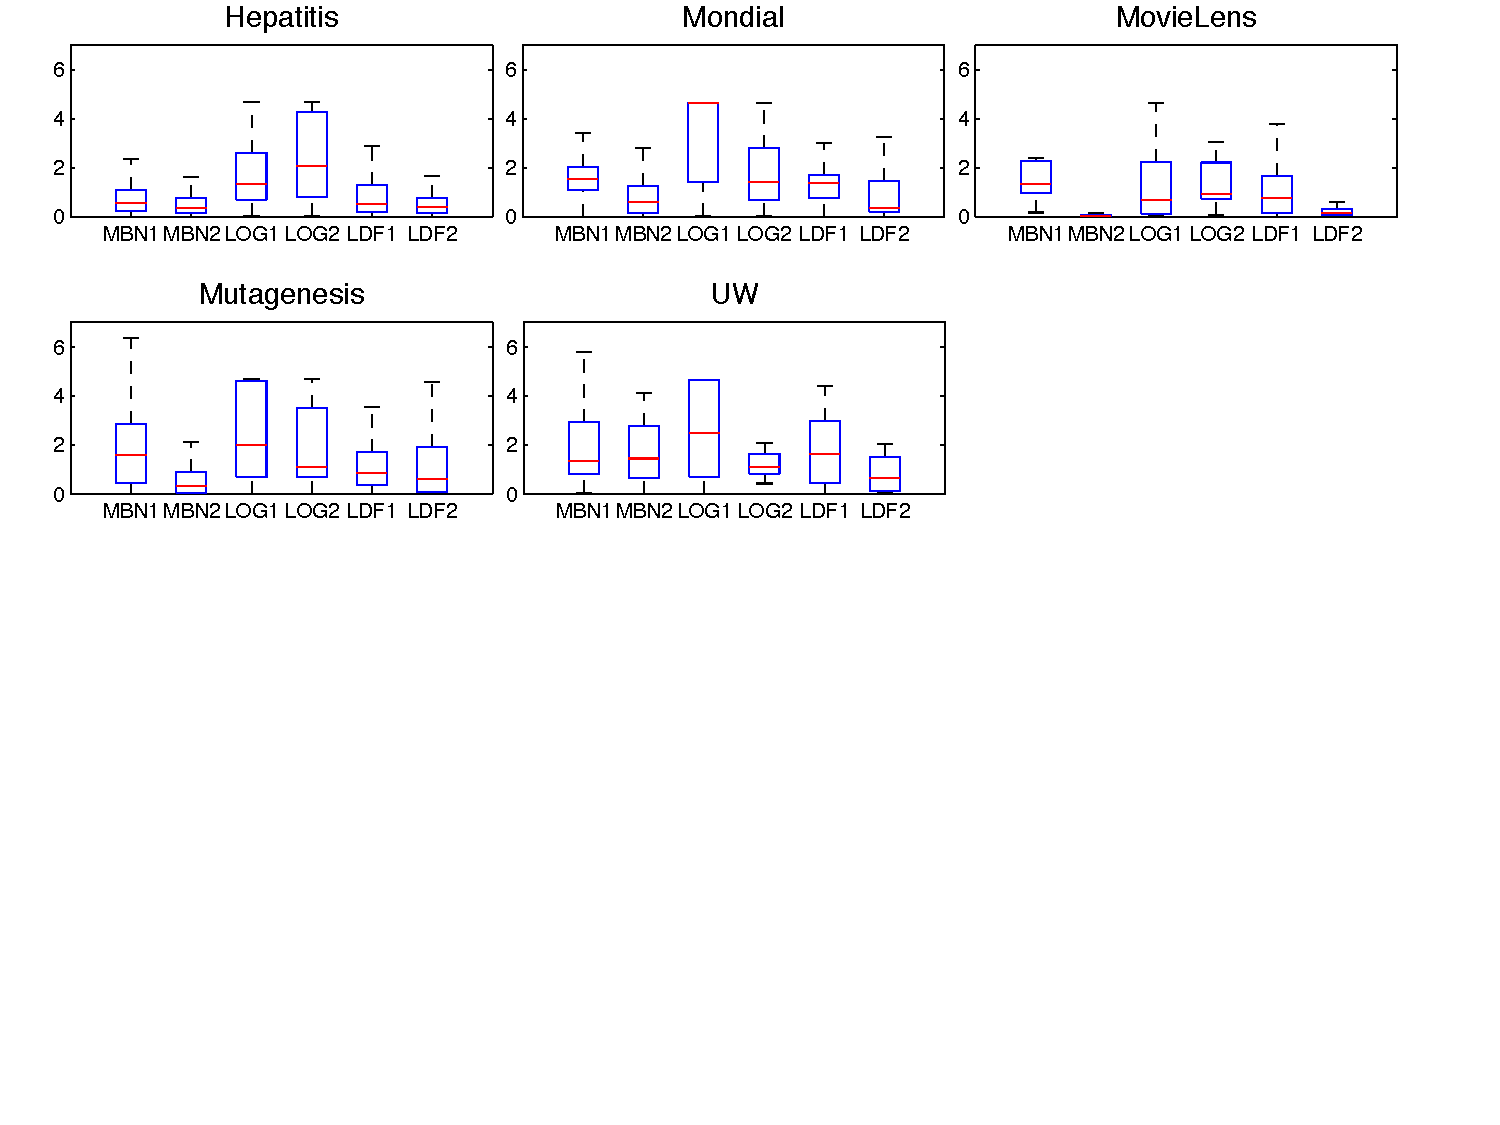
\includegraphics[width=1\textwidth]{boxplots}
%}
\caption{Boxplots of the absolute weight sizes from different weight learning methods. LOG=log(cp), LDF = log-diff. Method(i) is a box for (i)-variable formulas, for $i=1,2$. The box contains up to the 75th percentile of observed weights, the whisker up to the 95th percentile, and the line shows the median weight size.
\label{fig:boxplots}}
\end{center}
\end{figure*}

The optimized MBN-weights show clear scaling effects on every benchmark database. The strongest effect is in MovieLens and the weakest effect is in UW. This is evidence that optimal weights include a scaling component for balancing the different number of formula groundings. The log-difference weights also show scaling effects, which confirms our expectation that information from related entities is less important. 

\section{Proof of the Equivalence Theorem between frequency regression and random regression}

We begin by giving a definition of random regression using formal notation. Let us write $\population_{A}$ for the set of entities in the domain of a population variable (e.g., the set of students for $S$). Let $\A_{1},\ldots,\A_{m}$ be a list of {\em all} first-order variables that occur in the Markov blanket of target node $\Y$ in the regression graph for $\Y$. We write $\grounding$ to denote a simultaneous grounding of {\em each} variable $\A_{i}$. We write $\groundall$ for the space of all possible groundings of the variables in the Markov blanket; so $$\groundall = \population_{\A_{1}} \times \cdots \times \population_{\A_{m}}.$$ In the regression graph of Figure~3, there are 2 possible groundings of the population variable $\Y$, so $\groundall = \population_{\Y}$ and $|\groundall|=2.$
Applying $\grounding$ to a  functor node $\functor(\terms)$ with population variables defines a ground functor node $\grounding(\functor(\terms))$; to simplify notation, we write $\grounding(\functor)$ when the arguments to  the functor are not relevant. The notation $[\grounding(\functor(\terms))]_{\D}$ denotes the value determined by $\D$ when  $\functor$ is applied to ground term $\grounding(\terms)$.  For instance, $[\it{gender(Anna)}]_{\D} = W$ in the sample DB of Figure~1. When the notation is used with respect to a fixed database $\D$, we omit the $\D$ subscript. For a single $\grounding$, the unnormalized conditional Markov blanket probability is given by

\begin{equation} \label{eq:random-regress}
\tilde{P}_{\B}^{\grounding}(\Y = \y|\set{X}=\set{x}))=
\prod_{i} P_{\B}(\functor_{i} = [\grounding(\functor_{i})]| \parents_{i}=  [\grounding(\parents_{i})])
\end{equation}

where the index $i$ runs over the target node and its children. In the regression graph of Figure~3, the index runs over the set $\{\it{gender}(sam),\it{coffee\_{dr}(sam)}\}$.

Random regression is based on the expected value of the logarithm of this quantity,  over all possible equiprobable groundings, which is given by

\begin{equation} \label{eq:halpern-likelihood}
ln(\tilde{P}^{r}(\Y = \y|\set{X}=\set{x})) \equiv \frac{1}{|\groundall|} \sum_{\grounding \in \groundall} ln(P_{\B}^{\grounding}(\Y = \y|\set{X}=\set{x})).
\end{equation}

We are now ready to prove the equivalence of frequency regression and random regression.

\begin{theorem} \label{prop:randomize}
The frequency regression value  for a target node (Equation 5.2) equals the random regression value $n(\tilde{P}^{r}(\Y = \y|\set{X}=\set{x}))$. 
%; in symbols, $P^{r} = P^{\pseudo}$.
\end{theorem}

\begin{proof} {\em Notation.} We use the following expressions. Fix a target node $\Y$ with Markov blanket population variables $\A_{1},\ldots,\A_{m}$ and a database $\D$. Since $\Y$ is fixed, we omit the superscript $\Y$ from counting expressions like $\instances_{ijk}(\D)$.
For each family formula $\family_{ijk}$, where $i$ indexes the target node or a child of the target node, let $\grounding_{ijk}(\D)$ be the number of simultaneous groundings of all Markov blanket population variables that satisfy $\family_{ijk}$. Write $m_{i}$ for the number of possible groundings of the Markov blanket population variables that occur in family $\family_{ijk}$, and
 $r_{i}$ for the number of possible groundings of the Markov blanket population variables that  do {\em not} occur in $\family_{ijk}$ (if this set is empty, let $r_{i}:=1$.) For instance, if  $\A_{1},\A_{2}$ are the variables that occur in $\family_{ijk}$, then $m_{i} = |\population_{\X_{1}}| \times |\population_{\X_{2}}|$, and $r_{i} = \prod_{l=3}^{m}|\population_{\X_{l}}|$.
%| \cdots |\population_{\X_{k}}|$. 

Then we have

\begin{eqnarray*}
|\groundall| & = & m_{i} \cdot r_{i}\\
\grounding_{ijk}(\D) & = & \instances_{ijk}(\D) \cdot r_{i}
\end{eqnarray*}

Therefore $p_{ijk}(\D) = \instances_{ijk}(\D)/m_{i}=\gamma_{ijk}(\D)/|\groundall|$ and the frequency regression equation 3.2 can be written as

\begin{equation} \label{eq:simplify-pseudo}
 \sum_{ijk} p_{ijk}(\D) \cdot ln(\theta_{ijk}) = \frac{1}{|\groundall|} \sum_{ijk} \gamma_{ijk}(\D) \cdot ln(\theta_{ijk}).
\end{equation}
Each factor $ln(\theta_{ijk})$ in Equation~\eqref{eq:halpern-likelihood} appears in the sum $\sum_{\grounding \in \groundall}  ln(\tilde{P}_{\B}^{\grounding}(\Y = \y|\set{X}=\set{x}))$ once for each simultaneous grounding $\grounding \in \groundall$ that satisfies $\family_{ijk}$ in database $\D$. Therefore we have

\begin{equation} \label{eq:simplify-halpern}
\frac{1}{|\groundall|} \sum_{\grounding \in \groundall} ln(\tilde{P}_{\B}^{\grounding}(\D))= \frac{1}{|\groundall|} \sum_{ijk} \gamma_{ijk}(\D) \cdot ln(\theta_{ijk}).
\end{equation}

Equations~\eqref{eq:simplify-halpern} and~\eqref{eq:simplify-pseudo} together establish the identity of the random regression~\eqref{eq:halpern-likelihood} and frequency regression~3.2.
\end{proof}


\section{Proof of the Equivalence proposition between log-conditional weights and log-difference weights}
%\setcounter{proposition}{7}
\begin{proposition}
Frequency regression (Equation 5.2) returns the same result for log-conditional probability weights and for log-difference weights.
\end{proposition}

\begin{proof} In the following we fix an input database and therefore omit references to the database from the instance counts $\instances_{ijk}$ and frequencies $\prob_{ijk}$. Similarly we fix a target node $\Y$ and omit the superscript $\Y$. Then the frequency equation for the log-conditional parameters is
%\\$ln(\tilde{P}_{\it{cp}}(\Y = \y)) = \sum_{ijk} p_{ijk} \; ln(\theta_{ijk})$\\
$$ln(\tilde{P}_{\it{cp}}(\Y = \y)) = \sum_{ijk} p_{ijk} \; ln(\theta_{ijk})$$

and for the log-difference probabilities it is 
%
%\[ln(\tilde{P}_{\it{diff}}(\Y = \y)) =  \prob_{i0k} \; ln(\theta_{i0k}) + \sum_{ijk} p^{\Y}_{ijk} \; (ln(\theta_{ijk}) - ln(\theta_{i0k}))\]
\begin{small}
\begin{eqnarray*}
ln(\tilde{P}_{\it{diff}}(\Y = \y)) & & \\
= \sum_{ik} \prob_{i0k} \; ln(\theta_{i0k}) + \sum_{ijk} \prob_{ijk} \; (ln(\theta_{ijk}) - ln(\theta_{i0k})) && \\
=\sum_{ik} \prob_{i0k} \; ln(\theta_{i0k}) - \sum_{ijk} \prob_{ijk} \; ln(\theta_{i0k}) + ln(\tilde{P}_{\it{cp}}(\Y = \y)) && \\
%\scriptstyle 
=\sum_{ik} \prob_{i0k} \; ln(\theta_{i0k}) - \sum_{ik} ln(\theta_{i0k}) \sum_{j} \prob_{ijk} + ln(\tilde{P}_{\it{cp}}(\Y = \y)) && \\
=\sum_{ik} \prob_{i0k} \; ln(\theta_{i0k}) - \sum_{ik} ln(\theta_{i0k}) \; \prob_{i0k} + ln(\tilde{P}_{\it{cp}}(\Y = \y)) && \\
=ln(\tilde{P}_{\it{cp}}(\Y = \y))&&
%& = & \sum_{ik} \prob_{i0k} \; ln(\theta_{i0k}) - ln(\theta_{i0k}) \sum_{ijk} \prob_{ijk}  + ln(\tilde{P}_{\it{cp}}(\Y = \y))
\end{eqnarray*}
\end{small}
where the last-but-one equation follows 
%
%second equation follows from writing the summation of a difference as the difference of summations, and the third because the term $ln(\theta_{i0k})$ is constant throughout the summation. Focusing on the sum $\sum_{ijk} \prob_{ijk} \; ln(\theta_{i0k})$, we find that 
%
%\begin{eqnarray*} 
%\sum_{ijk} \prob_{ijk} \; ln(\theta_{i0k}) & = & \sum_{ik} ln(\theta_{i0k}) \sum_{j} \prob_{ijk} \\
%& = & \sum_{ik} ln(\theta_{i0k})\; \prob_{i0k}.
%\end{eqnarray*}
%
%The first equation follows because the term $ln(\theta_{i0k})$ does not depend on the parent state index $j$, and the second 
because summing out the parent states from the joint probabilities of child state and parent state yields the marginal probability of the child state. \end{proof}
%
%The first set of equations implies that  \[ln(\tilde{P}_{\it{cp}}(\Y = \y))- ln(\tilde{P}_{\it{diff}}(\Y = \y)) = \sum_{ik} \prob_{i0k} \; ln(\theta_{i0k}) - \sum_{ijk} \prob_{ijk} \; ln(\theta_{i0k})\] equals. The second set of equations implies that this difference is 0, which establishes the proposition.


% KEEP THIS: if we restrict to relevant relations, we can do the same proof conditional on the existence of a relationship. the only issue is if there are 0 groundings for all applicable formulas. In this case it's better to use log-diff, i.e., the true prior, rather than the uniform one.


\bibliographystyle{siam}
\bibliography{siam}

\end{document}